%
% PREAMBLE -- You do not need to change the following
%

\documentclass[12pt,letterpaper,oneside]{article}

% Font encoding
\usepackage[utf8]{inputenc}
\usepackage[T1]{fontenc}

% Required packages
\usepackage{palatino}
\usepackage{amsmath}
\usepackage{amsfonts}
\usepackage{amssymb}
\usepackage{siunitx}
\usepackage{csquotes}
\usepackage{enumerate}
\usepackage{microtype}
\usepackage{fancyhdr}
\usepackage{hyperref}
\usepackage{graphicx}
\usepackage{cleveref}

\usepackage[font=small,labelfont=bf]{caption}

\usepackage[sorting=none,style=authoryear]{biblatex}
\renewcommand*{\nameyeardelim}{\addcomma\space}
\addbibresource{bibliography.bib}

% Define some interesting math commands
\renewcommand{\vec}[1]{{\mathbf{#1}}}
\newcommand{\mat}[1]{{\mathbf{#1}}}
\newcommand{\T}{\ensuremath{\mathrm{T}}}

% Setup the page geometry
\usepackage[left=1in,right=1in,top=1in,bottom=0.75in,marginparwidth=0.6in]{geometry}
\setlength{\parindent}{0em}
\setlength{\parskip}{0.5em}
\renewcommand{\baselinestretch}{1.25}

% Setup the header
\pagestyle{fancy}
\fancyhead[L]{\projectCourse}
\fancyhead[C]{\projectShortName}
\fancyhead[R]{\projectStudentID}

% Define the "\MakeTitle" command
\newcommand{\MakeTitle}{%
	{%
		\thispagestyle{empty}
		\centering
		{\huge \projectName}
		\vfill
		{\large A Report Submitted in Partial Fulfillment of the Requirements for\\ \projectCourse}\\[1cm]
		{\large \projectStudentName}\\
		{\projectStudentID} \\[1cm]
		{\large \projectStudentFaculty}\\
		{\large \projectStudentDepartment}\\
		\vfill
		{\large \projectDate}\\[1cm]
		\emph{Course Instructor:}\\
		\projectCourseInstructor\\
		\vfill
		\includegraphics[width=0.5\textwidth]{\projectOrganizationLogo}
		\setcounter{page}{0}
		\newpage%
	}%
	{%
		\pagenumbering{roman}
		\setcounter{tocdepth}{2}
		\tableofcontents
		\newpage
		
		\setcounter{page}{0}
		\pagenumbering{arabic}
	}
}

%
% VARIABLES -- Changes these to your liking
%


\newcommand{\projectCourse}%
	{SYDE 556/750}
\newcommand{\projectCourseInstructor}%
	{Andreas Stöckel}
\newcommand{\projectOrganizationLogo}%
	{assets/uwlogo.pdf}
\newcommand{\projectName}%
	{An Exploration of a Biologically Plausible Project Report Template}
\newcommand{\projectShortName}%
	{State Prediction with Legendre Memory Units}
\newcommand{\projectTerm}%
	{Winter 2020}
\newcommand{\projectStudentName}%
	{Joane Doe}
\newcommand{\projectStudentID}%
	{0123456789}
\newcommand{\projectStudentFaculty}%
	{Faculty of Engineering}
\newcommand{\projectStudentDepartment}%
	{Department of Systems Design Engineering}
\newcommand{\projectDate}%
	{April 15, 2020}

%
% ACTUAL DOCUMENT -- Your content goes here
%

\begin{document}
	% Insert the title page and the table of contents
	\MakeTitle

	\section{Introduction}
	\label{sec:introduction}

	This project template is supposed to give you an idea of what a project report might look like. You do not have to follow this template in case you think that it is not well suited for your particular project. In particular, feel free to add more section headers or to skip some. Parts of this document are also meant as a quick \LaTeX tutorial.

	To get started quickly, you can, for example, upload the \enquote{\texttt{template.zip}} \href{https://github.com/astoeckel/syde556-w20/raw/master/project/template.zip}{ZIP file} located in the \texttt{project} folder in the course GitHub repository to an online service such as \href{https://www.overleaf.com/}{Overleaf}, which lets you edit \LaTeX documents without having to worry about installing the right tools on your computer. Of course, feel free to use any word processing tool you feel comfortable with.

	However, please make sure that you use similar formatting (12pt, preferably \enquote{Palatino} or \enquote{URW Palladio}, with 125\% line spacing, letter paper with 1 inch border). Your final report should \emph{be between (at least) ten and (at the very most) twenty content pages} (not counting the title page, table of contents, references; but counting figures and tables).

	You should use the introduction of your project report to introduce the reader to the problem domain and to motivate your project. Optimally, a reader reading your introduction should have the answers to the following questions in mind:
	\begin{itemize}
		\item What is your project about?
		\item Why is your project interesting? What problem does it solve?
		\item What is some prior work in the problem domain?
		\item What are your contributions?
		\item How is the rest of your project report structured?
	\end{itemize}

 	You might want to cite some relevant literature, such as \cite{eliasmith2003neural,eliasmith2013how}. To add more citations, edit the \texttt{bibliography.bib} file that is in the same directory as this template. Most academic publishers give you the opportunity to download a citations in the BibTeX format that is used within \texttt{bibliography.bib}. You can also consult the \texttt{bibliography.bib} file used in the lecture notes. Be careful when exporting BibTeX citations from Google Scholar, these are often incorrect or incomplete.
 	
 	You can use the \texttt{\textbackslash cite} command for an inline citation, such as \enquote{\cite{eliasmith2003neural}, point out that understanding how brains work is the most interesting human endeavor of all times.} Alternatively, put a citation in parentheses: \enquote{Building brains is the most interesting human endeavor of all times (\cite{eliasmith2003neural}).}

	\section{Neurobiological Model}

	Once you have finished the introduction (\Cref{sec:introduction}), and if your project is a modeling project, it might be useful to follow the steps outlined in \cite{eliasmith2003neural}: system description, design specification and implementation. Again, this is merely meant as a help for thinking about your project, not as a mandatory requirement.
	
	The next few subsections quickly summarize what each of these sections should contain, but have a look at the textbook for more details.

	\subsection{System Description}

	Try to gather as much information about the system your are trying to implement as possible, and think about how this information can be mapped onto the NEF (i.e., neuron populations representing state variables, transformations, and dynamics). This can encompass the following:
	\begin{enumerate}[1.]
		\item Connectivity between subsystems
		\item Neuron response functions
		\item Neuron tuning curves
		\item Relations between subsystems
		\item Overall system behavior
	\end{enumerate}

	\subsection{Design Specification}

	This is to specify the real-world constraints on the system even further. What is the range of values that each variable can take? What are the limits on the precision of these values? What are the dynamical characteristics (how fast is the system)?

	\subsection{Implementation}

	Here you can describe how you turned the system description and design specification into an actual model -- and depending on your project, it might be worthwhile to split \enquote{implementation} into its own section. You may show excerpts from your code, or a network diagram, or talk about the kind of software you used.

	If there are any, talk about the challenges that had to be overcome. Did you have to solve any interesting mathematical problems? If yes, you might want to write down some equations, such as \cref{eqn:example} below, which is as follows
	\begin{align}
		\big(\mat D^f\big)^\T &=  \arg\min_{\mat D^f} \frac{1}{|\mathbb{X}|} \int_{\mathbb{X}}  \| f(\vec x) - \mat D^f \vec a(\vec x)\|^2 \, \mathrm{d}\vec x \notag \\
			&= \big(\mat A \mat A^\T + N \sigma^2 \mat I \big)^{-1} \mat A \mat Y^\T
		\label{eqn:example}
	\end{align}
	where $\mat D^f$ is the function decoder for a neural ensemble.

	\section{Experiments and Results}

	\begin{figure}
		\centering
		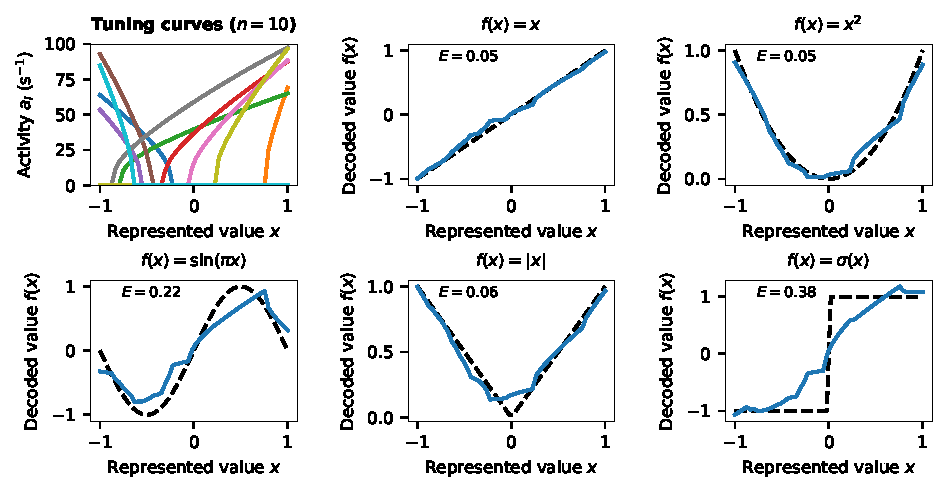
\includegraphics{media/function_decodings_10.pdf}
		\caption{For the figure caption, make sure to describe what the figure is showing, in particular any parts of the figure that are not immediately clear from the legend. Avoid interpreting your figures in the caption. Example: Function decodings for a neuron population with $n = 10$ neurons. The top-left figure shows the population tuning curves. In all other plots dashed lines correspond to the ideal function, blue lines to the function decoding. Depicted errors $E$ are the RMSE.}
		\label{fig:function_decodings_10.pdf}
	\end{figure}

	In the experiments and results section, you should, as the name suggests, \emph{describe} the experiments you are performing, followed by a \emph{description} of the results.

	The goal of an experiment is to \emph{quantify} whether the model you built is working as intended. For example, if your goal is to model a behavioural neurobiological system, you should measure the behaviour of the model and compare it to other data.

	Sometimes it is more suitable to interleave experiments, results and interpretation, i.e., you start with one experiment, describe the results, interpret the results, leading you to another experiments.

	Other times it might be more suitable to just describe all the experiments first, then list all the results, and to move the interpretation to a separate \enquote{discussion} section.

	It is up to you which style you think suites your project most.

	\section{Discussion and Conclusion}

	Feel free to split this section into two separate sections, whatever your think suits your project most.

	Overall, you should discuss your results. Did your model work as intended, on a qualitative (i.e., rough, overall behaviour) or even quantitative (i.e., the numbers match) level? What worked well and what did not?
	
	If things are not working as you have thought, try to come up with hypotheses as for why that is. Falsifying an initial hypothesis is not a failure! But you should make explicit what we can learn from such a failure.

	The conclusion should contain some information about potential future directions of research. Close with a final paragraph summarizing what you did and what we learned.

	\newpage
	\printbibliography
\end{document}